\chapter{Model Description}
\label{ch:model_description}

\epigraph{The purpose of abstraction is not to be vague, but to create a new semantic level in which one can be absolutely precise.}{--- Edsger W. Dijkstra}

\lettrine[lines=2]{T}{his chapter} presents the architecture of the agent-based model from the ground up: the spatial environment in which agents operate, the class hierarchy that organizes 18 agent types into a coherent inheritance tree, the paracrine effect system that mediates cell--cell signaling, the movement mechanics that govern spatial behavior, the step-by-step execution loop that advances the simulation, and the terminal conditions that determine patient outcomes.

% ============================================================================
\section{Spatial Environment}
\label{sec:md_spatial}
% ============================================================================

The simulation takes place on a three-dimensional discrete grid whose side length is derived from the patient's tumor volume.  Given a volume $V$ in cm$^3$ and a block size $\Delta = 10\;\mu\text{m}$, the grid dimension is
\begin{equation}
    L = \left\lfloor \frac{(V \times 10^{12})^{1/3}}{\Delta} \right\rfloor
    \label{eq:grid_dim}
\end{equation}
producing a cubic $L \times L \times L$ lattice (e.g., $L = 100$ for $V = 0.001\;\text{cm}^3$).  Multiple agents may occupy the same voxel; boundaries are \emph{sticky}.  A continuous glucose concentration field $C(\mathbf{x}, t) \in \mathbb{R}_{\geq 0}$ overlays the grid and evolves according to a reaction--diffusion equation (Chapter~\ref{ch:biological-subsystems}), providing the metabolic context for proliferation, killing, and chemotactic navigation.

% ============================================================================
\section{Agent Architecture}
\label{sec:md_architecture}
% ============================================================================

\subsection{Class Hierarchy}
\label{subsec:md_hierarchy}

The 18 agent types are organized into a four-level inheritance tree rooted at Repast4Py's \texttt{Agent} class (Figure~\ref{fig:agent_hierarchy}).  Two abstract base classes introduce the shared functionality that makes the hierarchy tractable.  \textbf{Cell} provides position tracking, deferred movement, effect collection, neighborhood queries, and duplication logic for every spatially embodied agent.  \textbf{TCell} extends \texttt{Cell} with T~lymphocyte-specific behaviors: a 16-bit TCR, antigen matching via Hamming distance ($d_H \leq 3$), hormone perception with exponential decay, and 17 sex-hormone modulation channels.  Five T~cell types inherit from \texttt{TCell}; eleven cellular agents inherit directly from \texttt{Cell}; and two non-cellular agents (\texttt{SexHormone}, \texttt{Cytokine}) inherit from the framework's \texttt{Agent} without spatial semantics.  Three cellular agents (\texttt{DendriticCell}, \texttt{PlasmacitoidDendriticCell}, \texttt{MacrophageM1}) additionally incorporate a \texttt{PhagocyticMixin} for antigen processing.

\begin{figure}[htbp]
\centering
\adjustbox{max width=0.85\textwidth, max height=0.7\textheight}{% Agent class hierarchy for the RCC agent-based model
% Wrapped externally in \adjustbox{max width=0.85\textwidth}
\begin{tikzpicture}[
  >=Stealth,
  every node/.style={
    rectangle, rounded corners=3pt, draw, align=center,
    minimum height=0.65cm, inner sep=4pt, font=\small
  },
  abstract/.style={fill=gray!20, dashed, draw=gray!70},
  tcellnode/.style={fill=treatment!15, draw=treatment!50},
  tumornode/.style={fill=tumorcell!15, draw=tumorcell!50},
  innatenode/.style={fill=immunecell!15, draw=immunecell!50},
  stromalnode/.style={fill=accent!15, draw=accent!50},
  bus/.style={thick, gray!60},
  arr/.style={->, thick, gray!60},
  annot/.style={draw=none, fill=none, minimum height=0pt, inner sep=1pt,
                font=\footnotesize\itshape},
]

% ===== Row 0: Root =====
\node[abstract] (root) at (5, 0) {\texttt{repast4py.Agent}};

% ===== Row 1: Cell + SexHormone / Cytokine =====
\node[abstract]    (cell)     at (2, -1.8) {\texttt{Cell}};
\node[stromalnode] (hormone)  at (11, -1.8) {\texttt{SexHormone}};
\node[stromalnode] (cytokine) at (11, -3.2) {\texttt{Cytokine}};

% Root -> level-1 bus
\draw[bus] (root.south) -- (5, -0.8);
\draw[bus] (2, -0.8) -- (11, -0.8);
\draw[arr] (2, -0.8) -- (cell.north);
\draw[arr] (11, -0.8) -- (hormone.north);
\draw[arr, dashed] (11, -0.8) -- (11, -1.2) -- (cytokine.north);

\node[annot] at (cell.west)      [left=2pt]  {abstract};
\node[annot] at (hormone.east)   [right=2pt] {immediate moves};
\node[annot] at (cytokine.east)  [right=2pt] {placeholder};

% ===== Row 2: Cell's direct children (first tier) =====
\coordinate (cbus) at (2, -2.7);
\draw[bus] (cell.south) -- (cbus);
\draw[bus] (-2.5, -2.7) -- (8, -2.7);

\node[abstract]   (tcell) at (-2.5, -3.8) {\texttt{TCell}};
\node[tumornode]  (tumor) at (0.2,  -3.8) {\texttt{TumorCell}};
\node[innatenode] (treg)  at (2.5,  -3.8) {\texttt{TregCell}};
\node[innatenode] (dc)    at (5,    -3.8) {\texttt{DendriticCell}};
\node[innatenode] (pdc)   at (8,    -3.8) {\texttt{PlasmacitoidDC}};

\foreach \n in {tcell, tumor, treg, dc, pdc} {
  \draw[arr] (\n.north |- cbus) -- (\n.north);
}

\node[annot] at (tcell.south) [below=1pt] {hormone perception, TCR};
\node[annot, font=\footnotesize\color{immunecell}] at (dc.south) [below=1pt]
     {+\,PhagocyticMixin};
\node[annot, font=\footnotesize\color{immunecell}] at (pdc.south) [below=1pt]
     {+\,PhagocyticMixin};

% ===== Row 3: Cell's direct children (second tier) =====
\coordinate (bus2drop) at (5, -2.7);
\coordinate (bus2) at (5, -5.4);
\draw[bus] (bus2drop) -- (bus2);
\draw[bus] (0.2, -5.4) -- (13.2, -5.4);

\node[innatenode]  (m1)     at (0.2,  -6.5) {\texttt{MacrophageM1}};
\node[innatenode]  (m2)     at (2.5,  -6.5) {\texttt{MacrophageM2}};
\node[innatenode]  (nk)     at (4.8,  -6.5) {\texttt{NaturalKiller}};
\node[innatenode]  (mast)   at (6.8,  -6.5) {\texttt{MastCell}};
\node[innatenode]  (neutro) at (8.8,  -6.5) {\texttt{Neutrophil}};
\node[stromalnode] (adipo)  at (10.8, -6.5) {\texttt{Adipocyte}};
\node[stromalnode] (blood)  at (13.2, -6.5) {\texttt{Blood}};

\foreach \n in {m1, m2, nk, mast, neutro, adipo, blood} {
  \draw[arr] (\n.north |- bus2) -- (\n.north);
}

\node[annot, font=\footnotesize\color{immunecell}] at (m1.south) [below=1pt]
     {+\,PhagocyticMixin};
\node[annot] at (blood.south) [below=1pt] {has\_step\,=\,False};

% ===== Row 3 (left): T-cell subclasses =====
\coordinate (tbusy) at (-2.5, -7.2);
\draw[bus] (tcell.south) -- ++(0, -1.3);
\draw[bus] (-8, -7.2) -- (3, -7.2);

\node[tcellnode] (cd8n) at (-8,   -8.3) {\texttt{CD8NaiveTCell}};
\node[tcellnode] (ctc)  at (-5.3, -8.3) {\texttt{CytotoxicTCell}};
\node[tcellnode] (cd4n) at (-2.5, -8.3) {\texttt{CD4NaiveTCell}};
\node[tcellnode] (th1)  at (0.3,  -8.3) {\texttt{CD4Helper1TCell}};
\node[tcellnode] (th2)  at (3,    -8.3) {\texttt{CD4Helper2TCell}};

\foreach \n in {cd8n, ctc, cd4n, th1, th2} {
  \draw[arr] (\n.north |- tbusy) -- (\n.north);
}

\node[annot] at (ctc.south) [below=1pt] {CD8+};
\node[annot] at (th1.south) [below=1pt] {Th1};
\node[annot] at (th2.south) [below=1pt] {Th2};

% ===== Legend (bottom-right) =====
\begin{scope}[shift={(11.5, -7.5)}]
  \node[draw=none, fill=none, font=\small\bfseries, minimum height=0pt,
        inner sep=0pt, anchor=north west] at (-0.2, 0) {Legend};
  \node[abstract, font=\footnotesize, minimum width=2.2cm]
        at (1, -0.6) {Abstract};
  \node[tcellnode, font=\footnotesize, minimum width=2.2cm]
        at (1, -1.3) {T~cells\,(5)};
  \node[tumornode, font=\footnotesize, minimum width=2.2cm]
        at (1, -2.0) {Tumor\,(1)};
  \node[innatenode, font=\footnotesize, minimum width=2.2cm]
        at (1, -2.7) {Innate\,(7)};
  \node[stromalnode, font=\footnotesize, minimum width=2.2cm]
        at (1, -3.4) {Stromal / signal\,(4)};
  \draw[gray!50, rounded corners=4pt]
        (-0.4, 0.3) rectangle (2.5, -3.8);
\end{scope}

\end{tikzpicture}
}
\caption{Agent class hierarchy.  Abstract bases are shown with dashed borders.  Color encodes functional category: T~cells (green), tumor (red), innate immune (blue), and stromal/signaling (orange).  Agents marked \emph{+\,PhagocyticMixin} gain a hunt--engulf--present state machine.}
\label{fig:agent_hierarchy}
\end{figure}

\FloatBarrier
\subsection{Agent Types}
\label{subsec:md_agent_types}

Table~\ref{tab:agent_types} lists all 18 agent types with their enumeration IDs and functional categories.  Each type is identified at runtime by an integer from the \texttt{AgentType} enumeration, enabling O(1) type checks during neighborhood queries and effect collection.

\begin{table}[htbp]
\centering
\caption{Agent types in the RCC model, with enumeration IDs and functional categories.}
\label{tab:agent_types}
{\footnotesize
\begin{tabular}{@{}clll@{}}
\toprule
\textbf{ID} & \textbf{Agent Type} & \textbf{Class Name} & \textbf{Category} \\
\midrule
0  & Tumor Cell            & \texttt{TumorCell}                   & Neoplastic \\
1  & Cytotoxic T Cell       & \texttt{CytotoxicTCell}              & Adaptive \\
2  & CD8$^+$ Na\"ive T Cell & \texttt{CD8NaiveTCell}               & Adaptive \\
3  & CD4$^+$ Na\"ive T Cell & \texttt{CD4NaiveTCell}               & Adaptive \\
4  & CD4$^+$ Th1 Cell       & \texttt{CD4Helper1TCell}             & Adaptive \\
5  & CD4$^+$ Th2 Cell       & \texttt{CD4Helper2TCell}             & Adaptive \\
6  & Regulatory T Cell      & \texttt{TregCell}                    & Adaptive \\
7  & Dendritic Cell         & \texttt{DendriticCell}               & Innate \\
8  & Plasmacytoid DC        & \texttt{PlasmacitoidDendriticCell}   & Innate \\
9  & M1 Macrophage          & \texttt{MacrophageM1}                & Innate \\
10 & M2 Macrophage          & \texttt{MacrophageM2}                & Innate \\
11 & Natural Killer         & \texttt{NaturalKiller}               & Innate \\
12 & Mast Cell              & \texttt{MastCell}                    & Innate \\
13 & Neutrophil             & \texttt{Neutrophil}                  & Innate \\
14 & Adipocyte              & \texttt{Adipocyte}                   & Stromal \\
15 & Blood Vessel           & \texttt{Blood}                       & Vasculature \\
16 & Sex Hormone            & \texttt{SexHormone}                  & Signaling \\
17 & Cytokine               & \texttt{Cytokine}                    & Signaling \\
\bottomrule
\end{tabular}
}
\end{table}

\FloatBarrier
\subsection{Behavioral Flags}
\label{subsec:md_flags}

Three boolean class-level flags govern loop participation: \texttt{has\_effect} (10 types emit paracrine effects), \texttt{needs\_effect} (8 types collect neighbor effects), and \texttt{has\_step} (all except \texttt{Blood}, which is static).  These flags let the model skip unnecessary work per tick.

% ============================================================================
\section{Agent Interactions}
\label{sec:md_interactions}
% ============================================================================

The 18 agent types interact through four principal mechanisms (Figure~\ref{fig:agent_interactions}). \emph{Cytotoxic killing}: CTLs, NK cells, M1 macrophages, and dendritic cells can directly destroy tumor cells, with kill probability modulated by the local effect field, glucose availability, and---for CTLs---TCR--neoantigen affinity (Hamming distance). \emph{Activation and differentiation}: dendritic cells activate na\"ive CD8$^+$ and CD4$^+$ T cells upon phagocytosis; activated CD8$^+$ cells become CTLs, while CD4$^+$ cells differentiate into Th1, Th2, or Treg depending on the local cytokine milieu. \emph{Immunosuppression}: Tregs suppress CTL killing ($-0.3$ on \param{t\_kill\_rate\_effect}) and DC phagocytosis; M2 macrophages shield tumor cells and promote angiogenesis; tumor cells themselves inhibit CTLs via PD-L1 (CD274-dependent). \emph{Promotion and recruitment}: Th1 cells recruit M1 macrophages and DCs; pDCs spawn NK cells; M2 macrophages promote angiogenesis; adipocytes drive M2 polarization.

\begin{figure}[htbp]
\centering
\adjustbox{max width=0.85\textwidth, max height=0.7\textheight}{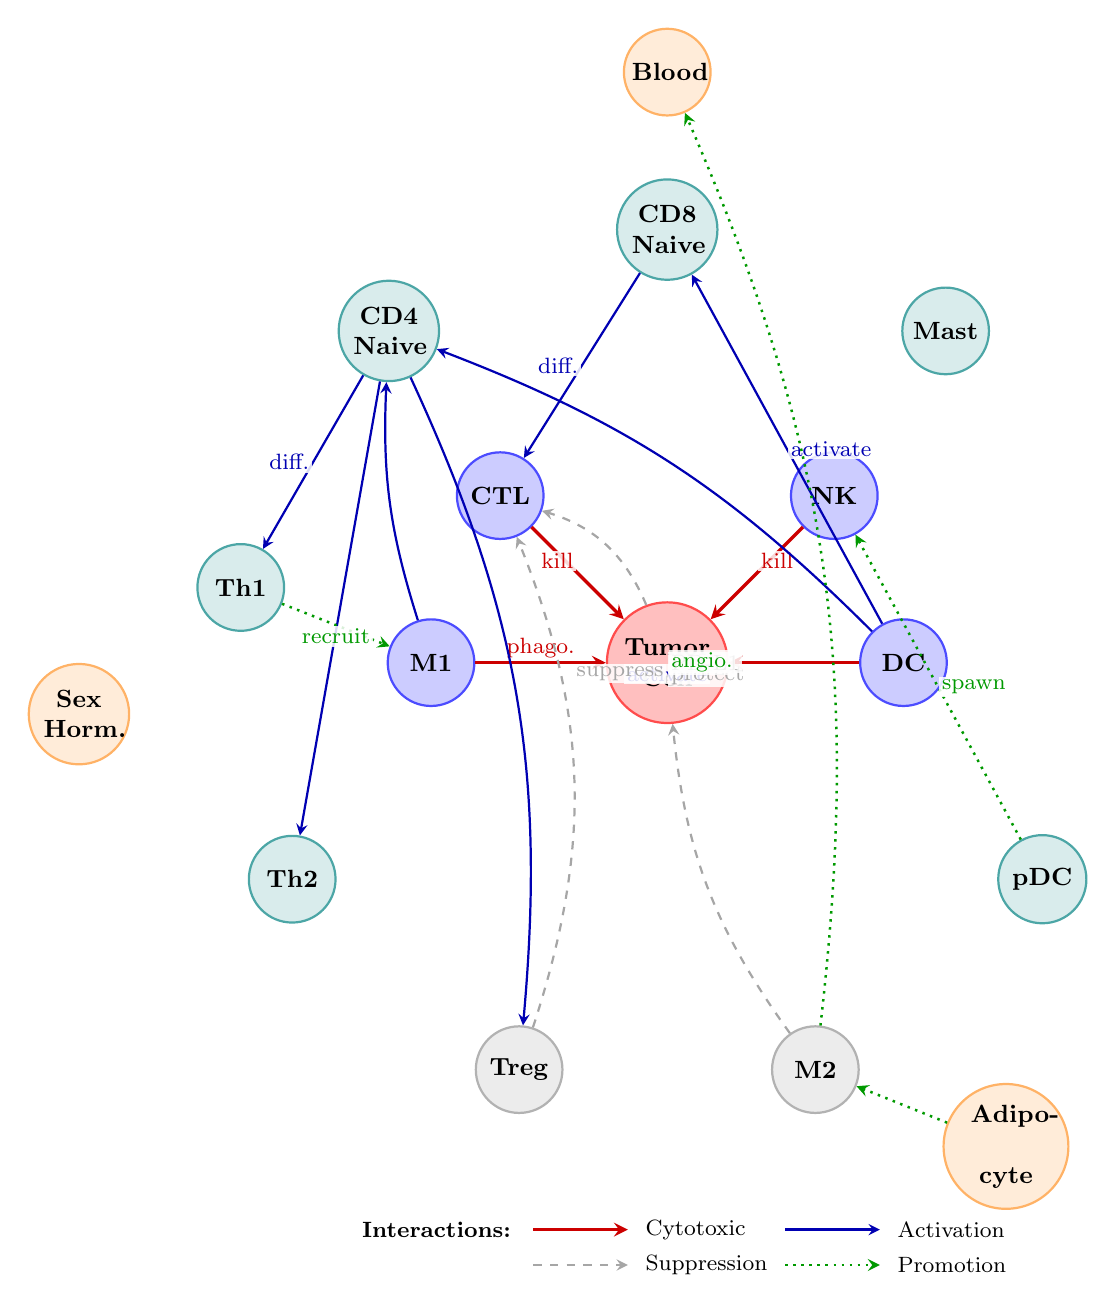
\begin{tikzpicture}[
  % Node styles
  agent/.style={circle, minimum size=1.1cm, text centered, font=\small, thick, inner sep=2pt},
  tumor/.style={agent, fill=red!25, draw=red!70, minimum size=1.4cm, text width=1.2cm},
  killer/.style={agent, fill=blue!20, draw=blue!70},
  adaptive/.style={agent, fill=teal!15, draw=teal!70, text width=0.9cm},
  regulatory/.style={agent, fill=gray!15, draw=gray!60},
  external/.style={agent, fill=orange!15, draw=orange!60, rounded corners=3pt, text width=0.9cm},
  % Edge styles
  cytotoxic/.style={->, >=stealth, red!80!black, line width=1.2pt},
  activation/.style={->, >=stealth, blue!70!black, line width=0.8pt},
  suppression/.style={->, >=stealth, gray!70, dashed, line width=0.8pt},
  promotion/.style={->, >=stealth, green!60!black, dotted, line width=0.9pt},
  % Label style
  lbl/.style={font=\footnotesize, fill=white, fill opacity=0.85, text opacity=1, inner sep=1pt},
]

% === CENTER: Tumor Cell ===
\node[tumor] (TC) at (0, 0) {\textbf{Tumor}\\\textbf{Cell}};

% === INNER RING (direct killers, r~3cm) ===
\node[killer] (CTL) at (135:3)  {\textbf{CTL}};
\node[killer] (NK)  at (45:3)   {\textbf{NK}};
\node[killer] (M1)  at (180:3)  {\textbf{M1}};
\node[killer] (DC)  at (0:3)    {\textbf{DC}};

% === OUTER RING (support/regulatory, r~5.5cm) ===
\node[adaptive]   (CD8N)  at (90:5.5)   {\textbf{CD8}\\\textbf{Naive}};
\node[adaptive]   (CD4N)  at (130:5.5)  {\textbf{CD4}\\\textbf{Naive}};
\node[adaptive]   (Th1)   at (170:5.5)  {\textbf{Th1}};
\node[adaptive]   (Th2)   at (210:5.5)  {\textbf{Th2}};
\node[regulatory] (Treg)  at (250:5.5)  {\textbf{Treg}};
\node[regulatory] (M2)    at (290:5.5)  {\textbf{M2}};
\node[adaptive]   (pDC)   at (330:5.5)  {\textbf{pDC}};
\node[adaptive]   (Mast)  at (50:5.5)   {\textbf{Mast}};

% === EXTERNAL (far out, r~7.5cm) ===
\node[external] (Blood)   at (90:7.5)   {\textbf{Blood}};
\node[external] (Hormone) at (185:7.5)  {\textbf{Sex}\\\textbf{Horm.}};
\node[external] (Adipo)   at (305:7.5)  {\textbf{Adipo-}\\\textbf{cyte}};

% ============================================================
% 1. CYTOTOXIC EDGES (red, solid, thick)
% ============================================================
\draw[cytotoxic] (CTL) -- (TC) node[lbl, midway, above left] {kill};
\draw[cytotoxic] (NK)  -- (TC) node[lbl, midway, above right] {kill};
\draw[cytotoxic] (M1)  -- (TC) node[lbl, midway, above] {phago.};
\draw[cytotoxic] (DC)  -- (TC);

% ============================================================
% 2. ACTIVATION / DIFFERENTIATION EDGES (blue, solid)
% ============================================================
\draw[activation] (DC)  -- (CD8N) node[lbl, midway, right] {activate};
\draw[activation] (DC)  to[bend right=12] (CD4N);
\draw[activation] (CD8N) -- (CTL) node[lbl, midway, left] {diff.};
\draw[activation] (CD4N) -- (Th1) node[lbl, midway, left] {diff.};
\draw[activation] (CD4N) -- (Th2);
\draw[activation] (CD4N) to[bend left=15] (Treg);
\draw[activation] (M1)  to[bend left=10] (CD4N) node[lbl, midway, below] {activate};

% ============================================================
% 3. SUPPRESSION EDGES (gray, dashed)
% ============================================================
\draw[suppression] (Treg) to[bend right=20] (CTL) node[lbl, midway, below left] {suppress};
\draw[suppression] (M2)   to[bend left=15] (TC)   node[lbl, midway, below right] {protect};
\draw[suppression] (TC)   to[bend right=25] (CTL)  node[lbl, pos=0.45, right] {PD-L1};

% ============================================================
% 4. PROMOTION EDGES (green, dotted)
% ============================================================
\draw[promotion] (Th1)  -- (M1)    node[lbl, midway, below] {recruit};
\draw[promotion] (pDC)  -- (NK)    node[lbl, midway, right] {spawn};
\draw[promotion] (M2)   to[bend right=15] (Blood) node[lbl, midway, right] {angio.};
\draw[promotion] (Adipo) -- (M2);

% ============================================================
% LEGEND (compact, bottom)
% ============================================================
\begin{scope}[yshift=-7.2cm, xshift=-0.5cm]
  \node[anchor=west, font=\footnotesize\bfseries] at (-3.5, 0) {Interactions:};
  % Cytotoxic
  \draw[cytotoxic] (-1.2, 0) -- (0, 0);
  \node[anchor=west, font=\footnotesize] at (0.1, 0) {Cytotoxic};
  % Activation
  \draw[activation] (2.0, 0) -- (3.2, 0);
  \node[anchor=west, font=\footnotesize] at (3.3, 0) {Activation};
  % Suppression
  \draw[suppression] (-1.2, -0.45) -- (0, -0.45);
  \node[anchor=west, font=\footnotesize] at (0.1, -0.45) {Suppression};
  % Promotion
  \draw[promotion] (2.0, -0.45) -- (3.2, -0.45);
  \node[anchor=west, font=\footnotesize] at (3.3, -0.45) {Promotion};
\end{scope}

\end{tikzpicture}}
\caption{Hub-and-spoke interaction network.  The tumor cell sits at the center; the inner ring contains the four direct killer types; the outer ring holds support and regulatory cells.  Edge color encodes interaction type: cytotoxic (red), activation (blue), suppression (grey dashed), and promotion (green dotted).}
\label{fig:agent_interactions}
\end{figure}

Table~\ref{tab:interactions} summarizes the key interactions by agent type.

\begin{table}[htbp]
\centering
\caption{Summary of agent interactions in the RCC model.}
\label{tab:interactions}
{\small
\begin{tabular}{@{}llp{6.5cm}@{}}
\toprule
\textbf{Agent} & \textbf{Role} & \textbf{Key Effects} \\
\midrule
TumorCell       & Neoplastic     & DNA-driven growth; PD-L1 evasion; 200$\times$ glucose uptake \\
CTL             & Cytotoxic      & TCR-matched killing; glucose/hormone-modulated \\
CD8/CD4 Na\"ive & Precursor      & Differentiate upon DC activation \\
Th1             & Pro-inflam.    & Recruits M1, DC; boosts tumor apoptosis \\
Th2             & Mixed          & Mild growth boost; recruits CTLs \\
Treg            & Suppressive    & Inhibits CTL ($-0.3$), proliferation, DC phagocytosis \\
DC              & APC            & Phagocytoses tumor; activates na\"ive T cells \\
pDC             & Specialized    & Spawns NK; boosts killing; promotes Treg diff. \\
M1              & Anti-tumor     & Phagocytoses tumor; boosts Th1; can polarize to M2 \\
M2              & Pro-tumor      & Inhibits killing; promotes growth \& angiogenesis \\
NK              & Innate cyto.   & Kills tumor; glucose-dependent \\
MastCell        & Dual role      & 50/50 pro-/anti-tumor phenotype per step \\
Neutrophil      & Sentinel       & Age-limited lifespan \\
Adipocyte       & Stromal        & Mild tumor promotion; M2 polarization \\
Blood           & Vasculature    & Glucose source; static; angiogenesis target \\
SexHormone      & Signaling      & 17 immune modulation channels \\
Cytokine        & Signaling      & Reserved for future extension \\
\bottomrule
\end{tabular}
}
\end{table}

% ============================================================================
\section{Effect System}
\label{sec:md_effects}
% ============================================================================

The paracrine effect system is the primary mechanism through which agents influence one another without direct contact.  Each \texttt{Cell} agent maintains an \texttt{experienced\_effects} object containing 14 floating-point fields (Figure~\ref{fig:effect_system}), grouped into five functional categories: T~cell modulation (4 fields controlling kill rate, proliferation, apoptosis, and activation), helper-specific effects (2 fields for Th1/Th2 proliferation), regulatory effects (3 fields governing Treg differentiation and M1/M2 macrophage polarization), tumor and vasculature effects (3 fields for tumor growth, apoptosis, and angiogenesis), and specialized effects (2 fields for DC phagocytosis and NK kill rate).

\subsection{Effect Production and Collection}
\label{subsec:md_effect_pipeline}

At each step, the model iterates over agents with \texttt{needs\_effect} set, querying the Moore neighborhood at radius~1, retrieving cached effect objects, and aggregating via element-wise addition.  The aggregation is additive: a Treg ($-0.3$ on kill rate) and an M1 macrophage ($+0.1$) near a CTL produce a net $-0.2$.  This superposition means no agent requires global knowledge; phenomena such as immune exclusion zones emerge from the spatial arrangement of producers.

\begin{figure}[htbp]
\centering
\adjustbox{max width=0.85\textwidth, max height=0.7\textheight}{% Effect System — Paracrine signaling in the RCC ABM
% Compile with: lualatex or pdflatex (requires tikz)
\begin{tikzpicture}[
    >=latex,
    node distance=0.35cm,
    % Box styles
    producer/.style={
        draw=orange!70!black, fill=orange!8, rounded corners=3pt,
        minimum width=3.6cm, minimum height=0.55cm,
        font=\small, align=center, text=orange!70!black
    },
    effectgroup/.style={
        draw=black!50, fill=gray!8, rounded corners=3pt,
        minimum width=3.8cm, font=\small, align=left,
        inner sep=5pt, text=black!80
    },
    consumer/.style={
        draw=blue!60!black, fill=blue!6, rounded corners=3pt,
        minimum width=3.0cm, minimum height=0.55cm,
        font=\small, align=center, text=blue!60!black
    },
    grouplabel/.style={
        font=\footnotesize\bfseries, text=black!70
    },
    bmibox/.style={
        draw=violet!60!black, fill=violet!6, rounded corners=3pt,
        font=\small, align=left, inner sep=6pt, text=violet!60!black
    },
    pipeline/.style={
        draw=black!40, fill=gray!4, rounded corners=3pt,
        font=\footnotesize, align=center, inner sep=5pt,
        text=black!70, dashed
    },
    arrow/.style={->, thick, color=black!50},
    warrow/.style={->, thick, color=orange!60!black},
    carrow/.style={->, thick, color=blue!50!black},
]

% =====================================================================
%  COLUMN 1 — EFFECT PRODUCERS (left)
% =====================================================================
\node[grouplabel] (plabel) at (0, 0) {Effect Producers};
\node[grouplabel] (plabel2) at (0, -0.35) {\footnotesize(\texttt{has\_effect = True})};

\node[producer, below=0.25cm of plabel2] (tumor)
    {\textbf{TumorCell}};
\node[producer, below=0.15cm of tumor, font=\footnotesize, minimum height=0.4cm] (tumor-eff)
    {growth\textsuperscript{+}, angiogenesis\textsuperscript{+}};

\node[producer, below=0.3cm of tumor-eff] (th1)
    {\textbf{Th1}};
\node[producer, below=0.15cm of th1, font=\footnotesize, minimum height=0.4cm] (th1-eff)
    {tumour\_apoptosis\textsuperscript{+}};

\node[producer, below=0.3cm of th1-eff] (th2)
    {\textbf{Th2}};
\node[producer, below=0.15cm of th2, font=\footnotesize, minimum height=0.4cm] (th2-eff)
    {t\_kill\_rate\textsuperscript{+}, growth\textsuperscript{+}};

\node[producer, below=0.3cm of th2-eff] (treg)
    {\textbf{Treg}};
\node[producer, below=0.15cm of treg, font=\footnotesize, minimum height=0.4cm,
      minimum width=3.6cm] (treg-eff)
    {kill\textsuperscript{$-$0.3}, prolif\textsuperscript{$-$}, activ\textsuperscript{$-$}, phago\textsuperscript{$-$}};

\node[producer, below=0.3cm of treg-eff] (nk)
    {\textbf{NK}};
\node[producer, below=0.15cm of nk, font=\footnotesize, minimum height=0.4cm] (nk-eff)
    {t\_kill\_rate\textsuperscript{+}};

\node[producer, below=0.3cm of nk-eff] (m1)
    {\textbf{M1}};
\node[producer, below=0.15cm of m1, font=\footnotesize, minimum height=0.4cm] (m1-eff)
    {t\_kill\_rate\textsuperscript{+}, th1\_prolif\textsuperscript{+}};

\node[producer, below=0.3cm of m1-eff] (m2)
    {\textbf{M2}};
\node[producer, below=0.15cm of m2, font=\footnotesize, minimum height=0.4cm] (m2-eff)
    {kill\textsuperscript{$-$}, growth\textsuperscript{+}, angio\textsuperscript{+}};

\node[producer, below=0.3cm of m2-eff] (pdc)
    {\textbf{pDC}};
\node[producer, below=0.15cm of pdc, font=\footnotesize, minimum height=0.4cm] (pdc-eff)
    {nkl\_kill\textsuperscript{+}, t\_kill\textsuperscript{+}, treg\_diff\textsuperscript{+}};

\node[producer, below=0.3cm of pdc-eff] (mast)
    {\textbf{Mast}};
\node[producer, below=0.15cm of mast, font=\footnotesize, minimum height=0.4cm] (mast-eff)
    {stochastic pro/anti (50/50)};

\node[producer, below=0.3cm of mast-eff] (adipo)
    {\textbf{Adipocyte}};
\node[producer, below=0.15cm of adipo, font=\footnotesize, minimum height=0.4cm] (adipo-eff)
    {growth\textsuperscript{+}, m2\_mutation\textsuperscript{+}};

% =====================================================================
%  COLUMN 2 — 14 EFFECT FIELDS (center)
% =====================================================================
% Position the central column to the right of the producers
\coordinate (ctr) at (6.5, -5.5);

\node[grouplabel] at (6.5, 0) (elabel) {14 Effect Fields};
\node[grouplabel] at (6.5, -0.35) (elabel2)
    {\footnotesize(per-cell \texttt{experienced\_effects} dict)};

% T-cell modulation group
\node[effectgroup, below=0.25cm of elabel2, minimum width=4.2cm] (g1) {%
    {\footnotesize\bfseries T-cell modulation (4)}\\[2pt]
    \footnotesize
    \textbullet~t\_kill\_rate\_effect\\
    \textbullet~t\_proliferation\_effect\\
    \textbullet~t\_apoptosis\_effect\\
    \textbullet~t\_activation\_effect
};

% Helper-specific group
\node[effectgroup, below=0.3cm of g1, minimum width=4.2cm] (g2) {%
    {\footnotesize\bfseries Helper-specific (2)}\\[2pt]
    \footnotesize
    \textbullet~th1\_proliferation\_effect\\
    \textbullet~th2\_proliferation\_effect
};

% Regulatory group
\node[effectgroup, below=0.3cm of g2, minimum width=4.2cm] (g3) {%
    {\footnotesize\bfseries Regulatory (3)}\\[2pt]
    \footnotesize
    \textbullet~treg\_differentiation\_effect\\
    \textbullet~m1\_mutation\_effect\\
    \textbullet~m2\_mutation\_effect
};

% Tumor group
\node[effectgroup, below=0.3cm of g3, minimum width=4.2cm] (g4) {%
    {\footnotesize\bfseries Tumor (3)}\\[2pt]
    \footnotesize
    \textbullet~tumour\_growth\_effect\\
    \textbullet~tumour\_apoptosis\_effect\\
    \textbullet~angiogenesis\_effect
};

% Specialized group
\node[effectgroup, below=0.3cm of g4, minimum width=4.2cm] (g5) {%
    {\footnotesize\bfseries Specialized (2)}\\[2pt]
    \footnotesize
    \textbullet~dc\_phagocytosis\_effect\\
    \textbullet~nkl\_kill\_rate\_effect
};

% =====================================================================
%  COLUMN 3 — EFFECT CONSUMERS (right)
% =====================================================================
\node[grouplabel] at (12, 0) (clabel) {Effect Consumers};
\node[grouplabel] at (12, -0.35) (clabel2)
    {\footnotesize(\texttt{needs\_effect = True})};

\node[consumer, below=0.25cm of clabel2] (c-tumor)  {\textbf{TumorCell}};
\node[consumer, below=0.2cm of c-tumor]  (c-cd8)    {\textbf{CD8Naive}};
\node[consumer, below=0.2cm of c-cd8]    (c-cd4)    {\textbf{CD4Naive}};
\node[consumer, below=0.2cm of c-cd4]    (c-ctl)    {\textbf{CytotoxicTCell}};
\node[consumer, below=0.2cm of c-ctl]    (c-th1)    {\textbf{Th1}};
\node[consumer, below=0.2cm of c-th1]    (c-m2)     {\textbf{M2}};
\node[consumer, below=0.2cm of c-m2]     (c-nk)     {\textbf{NK}};
\node[consumer, below=0.2cm of c-nk]     (c-dc)     {\textbf{DC}};

% =====================================================================
%  ARROWS: Producers → Effect Fields
% =====================================================================
% Gather a single connection point on the left edge of the central column
\foreach \src in {tumor-eff, th1-eff, th2-eff, treg-eff, nk-eff,
                  m1-eff, m2-eff, pdc-eff, mast-eff, adipo-eff}{
    \draw[warrow] (\src.east) -- ([xshift=-0.15cm]g3.west |- \src.east)
        -- (g3.west |- \src.east);
}

% Overarching label on the left arrows
\node[font=\footnotesize, text=orange!60!black, rotate=90, anchor=south]
    at (3.65, -5.5) {emit into Moore neighborhood};

% =====================================================================
%  ARROWS: Effect Fields → Consumers
% =====================================================================
\foreach \dst in {c-tumor, c-cd8, c-cd4, c-ctl, c-th1, c-m2, c-nk, c-dc}{
    \draw[carrow] (g3.east |- \dst.west) --
        ([xshift=0.15cm]g3.east |- \dst.west) -- (\dst.west);
}

% Overarching label on the right arrows
\node[font=\footnotesize, text=blue!50!black, rotate=90, anchor=north]
    at (9.65, -3.0) {\texttt{sum\_with()} aggregation};

% =====================================================================
%  COLLECTION PIPELINE (between columns, small annotation)
% =====================================================================
\node[pipeline, below=0.4cm of g5, minimum width=4.2cm] (pipe) {%
    \textbf{Collection pipeline}\\[2pt]
    Producer $\rightarrow$
    Moore neighborhood ($r{=}1$)\\
    $\rightarrow$ \texttt{sum\_with()} $\rightarrow$
    consumer \texttt{experienced\_effects}
};

% =====================================================================
%  BMI NORMALIZATION (bottom)
% =====================================================================
\node[bmibox, below=0.5cm of pipe, minimum width=7cm] (bmi) {%
    {\small\bfseries BMI Normalization}\\[3pt]
    \footnotesize
    4 fields receive BMI-derived baselines:\\[2pt]
    $\hat{B} = \dfrac{\mathrm{BMI} - \mu}{\sigma}$
    \quad with sex-specific $\mu, \sigma$\\[4pt]
    \textbullet~tumour\_growth\_effect
    \quad\textbullet~angiogenesis\_effect\\
    \textbullet~t\_kill\_rate\_effect
    \quad\textbullet~m2\_mutation\_effect
};

% Arrow from BMI box up to the effect fields
\draw[arrow, violet!60!black, dashed]
    (bmi.north) -- (pipe.south);

\end{tikzpicture}
}
\caption{The paracrine effect system.  Ten producer types (left) emit effects into the Moore neighborhood.  The 14 effect fields (center) accumulate via element-wise addition.  Eight consumer types (right) read the aggregated effects to modulate their behavior.  BMI normalization (bottom) provides baseline offsets for four fields.}
\label{fig:effect_system}
\end{figure}

\FloatBarrier
\subsection{BMI Normalization}
\label{subsec:md_bmi}

Four of the 14 effect fields receive BMI-dependent baseline offsets.  The normalized BMI $\hat{B} = (\text{BMI} - \mu)/\sigma$ uses sex-specific parameters ($\mu = 26.5$, $\sigma = 5.5$ for females; $\mu = 27.5$, $\sigma = 4.5$ for males).  The offset is applied as $\pm\hat{B} \times w_i$ to Treg differentiation ($-$), M1 polarization ($-$), M2 polarization ($+$), and NK kill rate ($-$).  A positive $\hat{B}$ (above-average BMI) therefore shifts the microenvironment toward immunosuppression---more M2, more Treg, less NK killing---consistent with clinical evidence linking obesity to poorer RCC prognosis.

% ============================================================================
\section{Movement Mechanics}
\label{sec:md_movement}
% ============================================================================

Spatial behavior in the model follows a two-phase \emph{deferred movement} pattern: during the agent-stepping phase, each agent computes its desired next position and stores it in \texttt{\_desired\_pos}; after all agents have stepped, the model batch-processes all pending moves in a single pass.  This ensures that every agent makes its movement decision based on the same spatial snapshot, eliminating bias from the random activation order.

\subsection{Directed Movement}
\label{subsec:md_directed}

The primary navigation method, \texttt{move\_towards()}, uses an expanding-radius search: it queries the spatial index at radii 1, 2, 4, 8, \ldots\ (doubling each iteration), finds the closest target by Manhattan distance $d_M(\mathbf{a}, \mathbf{b}) = |a_x - b_x| + |a_y - b_y| + |a_z - b_z|$, computes the normalized Euclidean direction vector, and moves one step along it (clamped to grid boundaries).  The doubling strategy guarantees $O(\log L)$ worst-case iterations.  The maximum search radius scales dynamically with tumor population as $\max(5,\; N_{\text{tumor}} / (10 \cdot w_{\text{search\_dim}}))$, allowing immune cells to detect growing tumor masses at increasing distances.

\FloatBarrier
\subsection{Glucose Chemotaxis}
\label{subsec:md_chemotaxis}

When an immune cell (CTL, M1, DC, or NK) fails to find a direct target, it may fall back to glucose chemotaxis.  With probability $w_{\text{glucose\_chemotaxis\_strength}}$, the agent queries the glucose field for the discretized gradient at its position:
\begin{equation}
    (\Delta x, \Delta y, \Delta z) = \operatorname{sign}\bigl(\nabla C(\mathbf{x})\bigr)
    \label{eq:chemotaxis}
\end{equation}
where the gradient is computed via central finite differences with Neumann (zero-flux) boundary conditions.  The agent then moves one step along the gradient direction, migrating toward glucose-rich regions---typically areas near blood vessels and active tumor growth fronts---providing a biologically plausible navigation strategy in the absence of direct antigen detection.

\FloatBarrier
\subsection{Sex Hormone Diffusion}
\label{subsec:md_hormone}

Sex hormone agents follow a \emph{non-deferred} movement model: each step, a hormone randomly selects (50/50) between biased diffusion away from vasculature (drift strength 0.25, weighting 26 Moore neighbors by Manhattan distance to the nearest blood vessel) and simple diffusion biased toward $+y$/$+z$ that removes the hormone upon grid exit.  Moves execute immediately since hormones do not depend on each other's positions.

Figure~\ref{fig:movement_mechanics} summarizes the complete movement decision process as a flowchart.

\begin{figure}[htbp]
\centering
\adjustbox{max width=0.85\textwidth, max height=0.7\textheight}{% Movement decision flowchart for RCC ABM agents
\begin{tikzpicture}[
  % Node styles
  process/.style={
    rectangle, rounded corners=4pt, draw=green!60!black, fill=green!10,
    text width=5.8cm, minimum height=1cm, align=center,
    font=\small, line width=0.8pt
  },
  decision/.style={
    diamond, draw=yellow!60!black, fill=yellow!15,
    text width=3.2cm, minimum height=1.2cm, align=center,
    font=\small, line width=0.8pt, inner sep=1pt,
    aspect=2
  },
  deferred/.style={
    rectangle, rounded corners=4pt, draw=blue!60!black, fill=blue!10,
    text width=5.8cm, minimum height=1cm, align=center,
    font=\small, line width=0.8pt
  },
  hormone/.style={
    rectangle, rounded corners=4pt, draw=orange!70!black, fill=orange!10,
    text width=5cm, minimum height=1cm, align=center,
    font=\small, line width=0.8pt
  },
  terminal/.style={
    rectangle, rounded corners=8pt, draw=red!60!black, fill=red!10,
    minimum width=2.4cm, minimum height=0.7cm, align=center,
    font=\small, line width=0.8pt
  },
  hormdecision/.style={
    diamond, draw=orange!70!black, fill=orange!10,
    text width=2.6cm, minimum height=1cm, align=center,
    font=\small, line width=0.8pt, inner sep=1pt,
    aspect=2
  },
  % Arrow style
  arr/.style={-{Stealth[length=5pt]}, line width=0.7pt},
  lbl/.style={font=\footnotesize, fill=white, inner sep=1.5pt}
]

% ===== Main column (left/center) =====

% Start
\node[terminal] (start) {Agent.step() called};

% Decision: has target type?
\node[decision, below=1.0cm of start] (hastarget)
  {Has target type?\\{\footnotesize (e.g.\ CTL $\to$ TumorCell)}};

% move_towards process
\node[process, below=1.2cm of hastarget] (movetowards)
  {\textbf{move\_towards()}\\[2pt]
   {\footnotesize Expanding radius search: $1, 2, 4, 8, \dots$ up to max\_radius}\\
   {\footnotesize Find closest target by Manhattan distance: $|\Delta x|{+}|\Delta y|{+}|\Delta z|$}\\
   {\footnotesize Compute normalized direction vector}\\
   {\footnotesize Scale by distance parameter (default\,=\,1)}\\
   {\footnotesize Clamp to grid boundaries}};

% Decision: target found?
\node[decision, below=1.0cm of movetowards] (targetfound)
  {Target found?};

% Set desired pos (target)
\node[deferred, below left=1.0cm and -0.5cm of targetfound] (setpos1)
  {Set \texttt{\_desired\_pos}\\{\footnotesize $\to$ Deferred movement (step 5)}};

% Decision: immune cell?
\node[decision, below=2.8cm of targetfound] (isimmune)
  {Immune cell?\\{\footnotesize (CTL, M1, DC, NK)}};

% Glucose chemotaxis
\node[process, below=1.2cm of isimmune] (chemotaxis)
  {\textbf{Glucose Chemotaxis}\\[2pt]
   {\footnotesize Roll probability: \texttt{random()} $<$ \texttt{w\_glucose\_chemotaxis\_strength}}\\
   {\footnotesize Compute discretized gradient: $\operatorname{sign}(\nabla C)$}\\
   {\footnotesize Move one step along gradient}};

% Set desired pos (chemotaxis)
\node[deferred, below=0.8cm of chemotaxis] (setpos2)
  {Set \texttt{\_desired\_pos}\\{\footnotesize $\to$ Deferred movement (step 5)}};

% Stay in place
\node[terminal, right=2.5cm of chemotaxis] (stay) {Stay in place};

% ===== Deferred movement phase (bottom) =====

\node[deferred, below=1.2cm of setpos2, text width=10cm] (deferphase)
  {\textbf{5. Deferred Movement Phase}\\[2pt]
   {\footnotesize Model iterates all agents with \texttt{\_desired\_pos} $\neq$ current pos}\\
   {\footnotesize Updates spatial index}\\
   {\footnotesize All decisions based on same spatial snapshot}};

\node[terminal, below=0.8cm of deferphase] (endmain) {Movement complete};

% ===== Hormone column (right) =====

\node[hormone, right=4.5cm of hastarget, yshift=0.5cm] (hormtitle)
  {\textbf{Special Case: Sex Hormone Diffusion}\\[2pt]
   {\footnotesize (Separate from agent movement)}};

\node[hormdecision, below=0.8cm of hormtitle] (hormcoin)
  {50/50 coin flip};

\node[hormone, below left=1.0cm and -0.8cm of hormcoin] (biased)
  {\textbf{Biased diffusion}\\[2pt]
   {\footnotesize Away from blood vessels}\\
   {\footnotesize drift\_strength = 0.25}};

\node[hormone, below right=1.0cm and -0.8cm of hormcoin] (simple)
  {\textbf{Simple diffusion}\\[2pt]
   {\footnotesize Biased toward $+y$/$+z$}};

\node[hormone, below=1.5cm of hormcoin, yshift=-1.8cm] (immhorm)
  {\textbf{Immediate move}\\{\footnotesize (not deferred---applied directly)}};

\node[hormdecision, below=0.8cm of immhorm] (oob)
  {Out of bounds?};

\node[terminal, below left=0.8cm and -0.3cm of oob] (remove)
  {Remove from\\simulation};

\node[terminal, below right=0.8cm and -0.3cm of oob] (hormend)
  {Hormone\\placed};

% ===== Arrows: Main column =====

\draw[arr] (start) -- (hastarget);

\draw[arr] (hastarget) -- node[lbl, right] {Yes} (movetowards);

\draw[arr] (movetowards) -- (targetfound);

\draw[arr] (targetfound) -| node[lbl, above left] {Yes} (setpos1);

% No target → fall through to immune check
\draw[arr] (targetfound.south) -- node[lbl, right] {No} (isimmune);

% No target type → fall through to immune check
\draw[arr] (hastarget.west) -| node[lbl, above, pos=0.25] {No}
  ([xshift=-1.8cm]isimmune.west) -- (isimmune.west);

\draw[arr] (isimmune) -- node[lbl, right] {Yes} (chemotaxis);

\draw[arr] (chemotaxis) -- (setpos2);

% Not immune → stay
\draw[arr] (isimmune.east) -| node[lbl, above, pos=0.25] {No} (stay);

% Deferred positions feed into deferred phase
\draw[arr] (setpos1.south) |- ([yshift=0.6cm]deferphase.north west) -- ([xshift=-2cm]deferphase.north);
\draw[arr] (setpos2) -- (deferphase);

\draw[arr] (deferphase) -- (endmain);

% ===== Arrows: Hormone column =====

\draw[arr] (hormtitle) -- (hormcoin);

\draw[arr] (hormcoin) -| node[lbl, above left] {50\%} (biased);
\draw[arr] (hormcoin) -| node[lbl, above right] {50\%} (simple);

\draw[arr] (biased) |- (immhorm);
\draw[arr] (simple) |- (immhorm);

\draw[arr] (immhorm) -- (oob);

\draw[arr] (oob) -| node[lbl, above left] {Yes} (remove);
\draw[arr] (oob) -| node[lbl, above right] {No} (hormend);

\end{tikzpicture}
}
\caption{Movement decision flowchart.  Cellular agents (left branch) attempt directed movement toward a target type, falling back to glucose chemotaxis if no target is found.  All cellular moves are deferred.  Sex hormones (right branch) use a biased random walk with immediate execution.}
\label{fig:movement_mechanics}
\end{figure}

% ============================================================================
\section{Simulation Step}
\label{sec:md_step}
% ============================================================================

Each call to \texttt{RCCModel.step()} advances the simulation by one discrete time unit through 13 operations executed in a fixed sequence (Figure~\ref{fig:simulation_pipeline}).  The ordering reflects three design constraints: (i) effects must be collected before agents act on them, (ii) treatment must be applied at the correct simulation time, and (iii) spatial updates must be deferred to prevent order-dependent artifacts.

\begin{enumerate}
    \item \textbf{Collect data.}  Record population counts by agent type, glucose field statistics (mean, min, max), and cumulative kill tallies.  These are written to the data log at the end of each step.

    \item \textbf{Check termination.}  Evaluate the four terminal conditions (Section~\ref{sec:md_terminal}).  If any is met, write the final log entry and halt the simulation.

    \item \textbf{Reset immune infiltration.}  Set the immune infiltration factor to 1 for Th1, Th2, and MastCell types, ensuring that these agents begin each step with a clean baseline before effects accumulate.

    \item \textbf{Apply effects.}  For each agent with \texttt{needs\_effect = True}, collect \texttt{Effect} objects from the Moore neighborhood (radius 1) and aggregate them into the agent's \texttt{experienced\_effects} via element-wise addition.

    \item \textbf{Treatment step.}  If the current step $t \geq t_{\text{start}}$, apply all active drug effects (ICI, TKI, or combination).  Drug mechanisms are detailed in Chapter~\ref{ch:treatment}.

    \item \textbf{Sex drift.}  Apply sex-dependent modulation to the CD8$^+$ na\"ive T~cell population: duplication for male patients, removal for female patients, with the magnitude decremented each step.

    \item \textbf{Glucose field step.}  Blood vessels inject glucose at cached positions; the field is diffused via a 3D discrete Laplacian ($6$-connected stencil, Neumann boundaries); natural decay reduces concentrations by factor $(1 - \lambda)$.

    \item \textbf{Manage blood.}  Evaluate angiogenesis conditions and spawn new blood vessels if warranted (minimum separation 30 cells, effect radius 3).  Refresh tumor cell blood access via breadth-first search from vessel-connected sources.

    \item \textbf{Update search dimension.}  Recompute the global cell search dimension as $\max(5,\; N_{\text{tumor}} / (10 \cdot w_{\text{search\_dim}}))$, ensuring that immune cells can detect tumors at ranges proportional to tumor burden.

    \item \textbf{Shuffle and step agents.}  Take a snapshot of all living agents with \texttt{has\_step = True}, shuffle randomly, and invoke each agent's \texttt{step()} method.  Agents set \texttt{\_desired\_pos} during this phase but are not yet moved.

    \item \textbf{Deferred movement.}  Batch-move all agents in the \texttt{\_pending\_moves} set whose \texttt{\_desired\_pos} differs from their current position, updating the spatial index in a single pass.

    \item \textbf{Spawn hormones.}  Generate sex hormone agents at blood vessel locations according to sex-specific hormone production probabilities.

    \item \textbf{Increment step counter.}  Advance $t \leftarrow t + 1$ and loop back to step~1.
\end{enumerate}

\begin{figure}[htbp]
\centering
\adjustbox{max width=0.85\textwidth, max height=0.7\textheight}{\begin{tikzpicture}[
  box/.style={rectangle, rounded corners, minimum width=2.8cm, minimum height=1cm, text centered, font=\footnotesize, draw=black, thick},
  databox/.style={box, fill=blue!15},
  processbox/.style={box, fill=green!15},
  agentbox/.style={box, fill=orange!15},
  controlbox/.style={box, fill=red!15},
  arrow/.style={->, >=stealth, thick, shorten >=2pt, shorten <=2pt},
  decision/.style={diamond, aspect=2, minimum width=2cm, minimum height=0.8cm, text centered, font=\tiny, draw=black, thick, fill=yellow!15}
]

% Main pipeline flow (vertical)
\node[databox] (collect) at (0, 8) {\textbf{1. Collect Data}\\Population counts\\Glucose statistics};

\node[decision] (terminate) at (0, 6.5) {\textbf{2. Check}\\Termination\\Conditions};

\node[processbox] (effects) at (0, 5) {\textbf{3. Apply Effects}\\Collect \& sum\\neighbor effects};

\node[controlbox] (treatment) at (0, 3.5) {\textbf{4. Treatment}\\ICI \& TKI\\drug effects};

\node[controlbox] (sexdrift) at (0, 2) {\textbf{5. Sex Drift}\\CD8+ modulation\\by sex};

\node[processbox] (glucose) at (0, 0.5) {\textbf{6. Glucose Step}\\Diffusion \& decay\\Blood injection};

\node[processbox] (blood) at (0, -1) {\textbf{7. Manage Blood}\\Angiogenesis\\BFS refresh};

\node[processbox] (search) at (0, -2.5) {\textbf{8. Search Dimension}\\Update cell\\search radius};

\node[agentbox] (agents) at (0, -4) {\textbf{9. Agent Steps}\\Individual agent\\behaviors (shuffled)};

\node[agentbox] (move) at (0, -5.5) {\textbf{10. Deferred Move}\\Batch movement\\Update positions};

\node[controlbox] (hormones) at (0, -7) {\textbf{11. Spawn Hormones}\\Sex hormone\\generation};

% Terminal paths
\node[controlbox] (log) at (4, 6.5) {\textbf{Write Log}\\\textbf{Terminate}};
\node[controlbox] (continue) at (-4, 5) {\textbf{Next Step}\\$t \leftarrow t+1$};

% Main flow arrows
\draw[arrow] (collect) -- (terminate);
\draw[arrow] (terminate) -- (effects);
\draw[arrow] (effects) -- (treatment);
\draw[arrow] (treatment) -- (sexdrift);
\draw[arrow] (sexdrift) -- (glucose);
\draw[arrow] (glucose) -- (blood);
\draw[arrow] (blood) -- (search);
\draw[arrow] (search) -- (agents);
\draw[arrow] (agents) -- (move);
\draw[arrow] (move) -- (hormones);

% Termination decision
\draw[arrow] (terminate) -- (log) node[midway, above] {\scriptsize yes};
\draw[arrow] (terminate) -- (effects) node[midway, right] {\scriptsize no};

% Loop back
\draw[arrow] (hormones) to [out=180, in=270] (continue);
\draw[arrow] (continue) to [out=90, in=180] (collect);

% Side annotations
\begin{scope}[xshift=6cm]
% Data collection details
\node[text width=3cm, font=\tiny, fill=gray!5, rounded corners, draw] at (0, 8) {
\textbf{Data collected:}\\
• Agent counts by type\\
• Glucose: mean, min, max\\
• Kill statistics\\
• Growth rates
};

% Termination conditions
\node[text width=3cm, font=\tiny, fill=gray!5, rounded corners, draw] at (0, 6) {
\textbf{Terminal conditions:}\\
• Max steps reached\\
• Tumor eliminated\\
• Tumor $>$ threshold\\
• Growth rate $>$ limit
};

% Agent behaviors
\node[text width=3cm, font=\tiny, fill=gray!5, rounded corners, draw] at (0, -4) {
\textbf{Agent behaviors:}\\
• Move towards targets\\
• Kill/proliferate\\
• Differentiate\\
• Apply hormones\\
• Set desired position
};
\end{scope}

% Parallel processes annotation
\begin{scope}[xshift=-6cm]
\node[text width=3cm, font=\tiny, fill=gray!5, rounded corners, draw] at (0, 0) {
\textbf{Glucose field:}\\
• 3D diffusion (PDE)\\
• Blood injection\\
• Cell consumption\\
• Natural decay\\
• Gradient computation
};

\node[text width=3cm, font=\tiny, fill=gray!5, rounded corners, draw] at (0, -2.5) {
\textbf{Spatial management:}\\
• Moore neighborhoods\\
• 3D distance queries\\
• BFS from blood vessels\\
• Deferred movement\\
• Collision handling
};
\end{scope}

% Time annotation
\node[text width=8cm, font=\footnotesize, text centered] at (0, -8.5) {
\textbf{One Simulation Step} --- Process repeats until termination condition met
};

\end{tikzpicture}}
\caption{The 13-step simulation loop.  Color encodes functional category: data and monitoring (blue), biological processes (green), agent execution (orange), and treatment (red).  Step~2 is a decision point that terminates the simulation if any terminal condition is satisfied.}
\label{fig:simulation_pipeline}
\end{figure}

% ============================================================================
\section{Terminal Conditions}
\label{sec:md_terminal}
% ============================================================================

The simulation terminates when any of four conditions is met: maximum steps reached ($t \geq t_{\max}$, death), tumor elimination (count $= 0$, survival), critical mass ($\geq 2000$ cells, death), or uncontrolled growth ($\bar{G} \geq w_{\text{growth\_threshold}}$, death).  The growth metric is
\begin{equation}
    \bar{G} = \frac{1}{N_T} \sum_{i=1}^{N_T} \sigma\bigl(g_i + a_i;\; k{=}10\bigr)
    \label{eq:growth_rate}
\end{equation}
combines effect-driven growth, DNA-derived proliferation, blood access, and apoptosis components.  This last condition detects rapid acceleration even when absolute cell counts remain below critical mass.

With the model's spatial, behavioral, and interaction architecture established, the next chapter examines the three biological subsystems---glucose metabolism, DNA mutation, and sex hormones---that drive the emergent dynamics within this framework.
